\begin{enumerate}[label=\thechapter.\arabic*,ref=\thechapter.\theenumi]
	\item Consider the experiment of throwing a die.
    \begin{itemize}
        \item If a multiple of 3 comes up, throw the die again
        \item If any other number comes, toss a coin.
    \end{itemize}
     Find the conditional probability of the event \lq the coin shows a tail\rq, given that \lq at least one die shows a 3\rq.\\
		\iffalse
\documentclass[journal,12pt,two column]{IEEEtran}
%\usepackage{setspace}
\usepackage{listings}
\usepackage{amssymb}
\usepackage[cmex10]{amsmath}
\usepackage{amsthm}
\usepackage[export]{adjustbox}
\usepackage{bm}
\def\inputGnumericTable{} 

\usepackage[latin1]{inputenc}                                 
\usepackage{color}                                            
\usepackage{array} 
\usepackage{longtable} 
\usepackage{calc}                                             
\usepackage{multirow}                                         
\usepackage{hhline}                                           
\usepackage{ifthen}  
\usepackage{mathtools}
\usepackage{tikz}
\usepackage{listings}
\usepackage{color}                                            %%
\usepackage{array}                                            %%
\usepackage{caption} 
\usepackage{graphicx}

\title{A1110 Assignment 3 \\ 12.13.1.15}
\author{K.SaiTeja \\ AI22BTECH11014}
\providecommand{\pr}[1]{\ensuremath{\Pr\left(#1\right)}}
\providecommand{\qfunc}[1]{\ensuremath{Q\left(#1\right)}}
\providecommand{\sbrak}[1]{\ensuremath{{}\left[#1\right]}}
\providecommand{\lsbrak}[1]{\ensuremath{{}\left[#1\right.}}
\providecommand{\rsbrak}[1]{\ensuremath{{}\left.#1\right]}}
\providecommand{\brak}[1]{\ensuremath{\left(#1\right)}}
\providecommand{\lbrak}[1]{\ensuremath{\left(#1\right.}}
\providecommand{\rbrak}[1]{\ensuremath{\left.#1\right)}}
\providecommand{\cbrak}[1]{\ensuremath{\left\{#1\right\}}}
\providecommand{\lcbrak}[1]{\ensuremath{\left\{#1\right.}}
\providecommand{\rcbrak}[1]{\ensuremath{\left.#1\right\}}}
\newcommand*{\permcomb}[4][0mu]{{{}^{#3}\mkern#1#2_{#4}}}
\newcommand*{\perm}[1][-3mu]{\permcomb[#1]{P}}
\newcommand*{\comb}[1][-1mu]{\permcomb[#1]{C}}

\renewcommand{\thetable}{\arabic{table}} 
\newcommand{\question}{\noindent \textbf{Question: }}	
\newcommand{\solution}{\noindent \textbf{Solution: }}
\providecommand{\mbf}{\mathbf}
\providecommand{\pr}[1]{\ensuremath{\Pr\left(#1\right)}}
\providecommand{\prt}[2]{\ensuremath{P_{#1}^{\left(#2\right)} }}        % own macro for this question
\providecommand{\qfunc}[1]{\ensuremath{Q\left(#1\right)}}
\providecommand{\sbrak}[1]{\ensuremath{{}\left[#1\right]}}      % []
\providecommand{\lsbrak}[1]{\ensuremath{{}\left[#1\right.}}
\providecommand{\rsbrak}[1]{\ensuremath{{}\left.#1\right]}}
\providecommand{\brak}[1]{\ensuremath{\left(#1\right)}}         % ()
\providecommand{\lbrak}[1]{\ensuremath{\left(#1\right.}}
\providecommand{\rbrak}[1]{\ensuremath{\left.#1\right)}}
\providecommand{\cbrak}[1]{\ensuremath{\left\{#1\right\}}}      % {}
\providecommand{\lcbrak}[1]{\ensuremath{\left\{#1\right.}}
\providecommand{\rcbrak}[1]{\ensuremath{\left.#1\right\}}}
\theoremstyle{remark}
\newtheorem{rem}{Remark}
\newcommand{\sgn}{\mathop{\mathrm{sgn}}}
\providecommand{\abs}[1]{\ensuremath{\left\vert#1\right\vert}}
\providecommand{\res}[1]{\Res\displaylimits_{#1}} 
\providecommand{\norm}[1]{\ensuremath{\left\lVert#1\right\rVert}}
%\providecommand{\norm}[1]{\lVert#1\rVert}
\providecommand{\mtx}[1]{\mathbf{#1}}
\providecommand{\mean}[1]{\ensuremath{E\left[ #1 \right]}}
\providecommand{\fourier}{\overset{\mathcal{F}}{ \rightleftharpoons}}
%\providecommand{\hilbert}{\overset{\mathcal{H}}{ \rightleftharpoons}}
\providecommand{\system}{\overset{\mathcal{H}}{ \longleftrightarrow}}
	%\newcommand{\solution}[2]{\textbf{Solution:}{#1}}
\newcommand{\cosec}{\,\text{cosec}\,}
\providecommand{\dec}[2]{\ensuremath{\overset{#1}{\underset{#2}{\gtrless}}}}
\newcommand{\myvec}[1]{\ensuremath{\begin{pmatrix}#1\end{pmatrix}}}
\newcommand{\mydet}[1]{\ensuremath{\begin{vmatrix}#1\end{vmatrix}}}
%
%not used because document is short:
%\numberwithin{equation}{section}
%\numberwithin{figure}{section}
%\numberwithin{table}{section}
%\numberwithin{equation}{section}
%\numberwithin{problem}{section}
%\numberwithin{definition}{section}
\makeatletter
\@addtoreset{figure}{problem}
\makeatother

\let\StandardTheFigure\thefigure
\let\vec\mathbf
%\renewcommand{\thefigure}{\theproblem.\arabic{figure}}
    %\renewcommand{\thefigure}{\theproblem}
%\setlist[enumerate,1]{before=\renewcommand\theequation{\theenumi.\arabic{equation}}
%\counterwithin{equation}{enumi}
%\renewcommand{\theequation}{\arabic{subsection}.\arabic{equation}}

\def\putbox#1#2#3{\makebox[0in][l]{\makebox[#1][l]{}\raisebox{\baselineskip}[0in][0in]{\raisebox{#2}[0in][0in]{#3}}}}
     \def\rightbox#1{\makebox[0in][r]{#1}}
     \def\centbox#1{\makebox[0in]{#1}}
     \def\topbox#1{\raisebox{-\baselineskip}[0in][0in]{#1}}
     \def\midbox#1{\raisebox{-0.5\baselineskip}[0in][0in]{#1}}
\vspace{3cm}

%\renewcommand{\thefigure}{\theenumi}
%\renewcommand{\thetable}{\theenumi}
%\renewcommand{\theequation}{\theenumi}

\begin{document}
\maketitle
\question
\solution\tableofcontents
\fi
\begin{enumerate}
	\item  See 
        \tabref{tab:ncert/12/13/1/15m/States}	
	and 
        \figref{fig:ncert/12/13/1/15m/ markov_chain}.
    \begin{table}[ht!]
        \centering
    	%%%%%%%%%%%%%%%%%%%%%%%%%%%%%%%%%%%%%%%%%%%%%%%%%%%%%%%%%%%%%%%%%%%%%%
%%                                                                  %%
%%  This is a LaTeX2e table fragment exported from Gnumeric.        %%
%%                                                                  %%
%%%%%%%%%%%%%%%%%%%%%%%%%%%%%%%%%%%%%%%%%%%%%%%%%%%%%%%%%%%%%%%%%%%%%%

\begin{center}
\begin{tabular}{|c|c|c|}
\hline
\textbf{RV}& \textbf{Values} & \textbf{Description} \\ \hline
$X$		   & 	$\{0,1\}$	&  1st draw - 0: Red, 1: Black\\ \hline
$Y$ 		   & 	$\{0,1\}$	&  2nd draw - 0: Red, 1: Black\\ \hline
\end{tabular}
\end{center}

        \caption{States in Markov Chain}
        \label{tab:ncert/12/13/1/15m/States}	
    \end{table}
\begin{figure}[!ht]
        \centering
        \input{ncert/12/13/1/15m/figs/graph1.tex}  
        \caption{Graph of Markov Chain}
        \label{fig:ncert/12/13/1/15m/ markov_chain}
\end{figure}
\item 
    The state vector is,   
    \begin{align}
        \vec{Q}_n &= \myvec{\prt{0}{n}\\ 
        			        \prt{1}{n} \\
        			        \prt{2}{n} \\
        			        \prt{3}{n} 
        			        }        
    \end{align}    
    The probabilities after one step in time are
    \begin{align}
       \prt{0}{n+1} &= \frac{2}{6} \times \prt{0}{n}  \\
       \prt{1}{n+1} &= \frac{4}{6} \times \prt{0}{n}  \\
       \prt{2}{n+1} &= \frac{1}{2} \times \prt{1}{n} + 1 \times \prt{2}{n}
\\
       \prt{3}{n+1} &= \frac{1}{2} \times \prt{1}{n} + 1 \times \prt{3}{n} 
    \end{align}
   \item  
    The previous equations can be summarized as
    \begin{align}
        \vec{Q}_{n+1} &= \vec{P}\vec{Q}_n 
        \label{eq:ncert/12/13/1/15m/transtition}        
    \end{align}
		Where $\vec{P}$ is the transition probability matrix. Its elements are values of $p_{i|j}$
    \begin{align}
        \vec{P}= \myvec{%%%%%%%%%%%%%%%%%%%%%%%%%%%%%%%%%%%%%%%%%%%%%%%%%%%%%%%%%%%%%%%%%%%%%%
%%                                                                  %%
%%  This is a LaTeX2e table fragment exported from Gnumeric.        %%
%%                                                                  %%
%%%%%%%%%%%%%%%%%%%%%%%%%%%%%%%%%%%%%%%%%%%%%%%%%%%%%%%%%%%%%%%%%%%%%%

\begin{center}
\begin{tabular}{|c|c|}
\hline
\textbf{Event}& \textbf{Probability} \\ \hline
$\pr{A = 1}$ & 	$\frac{4}{5}$ \\ \hline
$\pr{X = 1}$ & 	$\frac{1}{2}$ \\ \hline
$\pr{X = 1 \mid A= 1}$ &  $\frac{1}{2}$ \\ \hline
\end{tabular}
\end{center}
} 
    \end{align}
\item 
     The given condition is that \lq3 occurs at least once\rq. Let the first occurrence of 3 be the initial state $ \vec{Q}_0$.
    \begin{align}
        \vec{Q}_0 &= \myvec{ 1 \\ 0 \\ 0 \\ 0 } 
    \end{align}
    Using \eqref{eq:ncert/12/13/1/15m/transtition}, further states can be generated.
    \begin{align}
        \vec{Q}_1 &= \vec{P} \vec{Q}_0
            = \myvec{\frac{2}{6} \\[4pt] \frac{4}{6}  \\[4pt] 0 \\ 0}\\
        \vec{Q}_2 &= \vec{P} \vec{Q}_1 = \vec{P}^{2} \vec{Q}_0 
            = \myvec{\frac{4}{9}  \\[4pt] \frac{8}{9}  \\[4pt] \frac{5}{24}\\[4pt] \frac{5}{12}} \\   
        \vdots \\
        \vec{Q}_n &= \vec{P}^{n} \vec{Q}_0
    \end{align}
    \item 
 Now to find the eigen values, 
 \begin{align}
\mydet{\vec{P}-\lambda \vec{I}} &= 0  
\\
 \implies \myvec{\input{ncert/12/13/1/15m/tables/table4.txt}} &= 0
 \\
	 \implies \lambda\brak{\frac{2}{6} - \lambda}\brak{1 - \lambda^2} &= 0
	 \\
	 \text{or, }\lambda &= \frac{2}{6}, 0 , 1 , 1 
 \end{align}
 The corresponding eigenvectors are
\begin{enumerate}
\item $\lambda = \frac{2}{6}$
\begin{align}
\vec{X} &= \myvec{\frac{-2}{3}\\[4pt] \frac{-4}{3}\\[4pt] 1\\[4pt] 1}
\end{align}
\item $\lambda = 0$
\begin{align}
\vec{X} &= \myvec{0 \\[2pt] -2\\[2pt] 1\\ 1}
\end{align}
\item $\lambda = 1$
\begin{align}
\vec{X} &= \myvec{0 \\ 0 \\ 1 \\ 0},\, 
\myvec{0 \\ 0 \\ 0 \\ 1}\\
\end{align}
\end{enumerate}
resulting in the 
eigenvector matrix
\begin{align}
\vec{S} &= \myvec{\input{ncert/12/13/1/15m/tables/table5.txt}}
\end{align}
Thus, 
\begin{align}
	\vec{P} &= \vec{S}\vec{D}\vec{S}^{-1}
\end{align}
Where $\vec{D}$ is eigenvalue matrix
\begin{align}
\vec{D} &= \myvec{\input{ncert/12/13/1/15m/tables/table6.txt}}
\end{align}
\item
\begin{align}
\vec{P}^{n} &= (\vec{S}\vec{D}\vec{S}^{-1})(\vec{S}\vec{D}\vec{S}^{-1}) \dots (\vec{S}\vec{D}\vec{S}^{-1})\\
\implies  &= \vec{S}\vec{D}^{n}\vec{S}^{-1}\\
\implies \lim_{n \to \infty}\vec{P}^{n} &= \lim_{n \to \infty}\vec{S}\vec{D}^{n}\vec{S}^{-1}
\end{align}
	From 
        \eqref{eq:ncert/12/13/1/15m/transtition},
\begin{align}
\vec{Q}_{n} &= \vec{P}^{n}\vec{Q}_{0}
\end{align}
and
Now,
\begin{align}
\vec{\lim_{n \to \infty}\vec{D}^{n}} &= \myvec{\input{ncert/12/13/1/15m/tables/table7.txt}}\\ 
\implies \vec{\lim_{n \to \infty}\vec{S}\vec{D}^{n}\vec{S}^{-1}} &= \myvec{\input{ncert/12/13/1/15m/tables/table7.txt}} = \vec{\vec{P}^{n}}\\
\implies \vec{Q}_n &= \myvec{\input{ncert/12/13/1/15m/tables/table7.txt}}\vec{Q}_0\\
\implies \vec{Q}_n &= \myvec{0 \\ 0 \\ 0 \\ 0} 
\end{align}
\item 
    Probability of the coin showing tails, given that at least one die shows a 3,
    \begin{align}
       \lim_{n \to \infty} \prt{3}{n} = 0
    \end{align}
   \end{enumerate} 

  \item
  A and B throw a pair of dice alternately. A wins the game if he gets a total of
6 and B wins if she gets a total of 7. It A starts the game, find the probability of
winning the game by A in third throw of the pair of dice.
\iffalse
\documentclass[book,11pt]{IEEEtran}
\usepackage{setspace}
\usepackage{gensymb}
\singlespacing
\usepackage[cmex10]{amsmath}
\usepackage{amsthm}
\usepackage{mathrsfs}
\usepackage{txfonts}
\usepackage{stfloats}
\usepackage{bm}
\usepackage{cite}
\usepackage{cases}
\usepackage{subfig}
\usepackage{longtable}
\usepackage{multirow}
\usepackage{enumitem}
\usepackage{mathtools}
\usepackage{tikz}
\usepackage{circuitikz}
\usepackage{verbatim}
\usepackage[breaklinks=true]{hyperref}
\usepackage{tkz-euclide} % loads  TikZ and tkz-base
\usepackage{listings}
\usepackage{color}    
\usepackage{array}    
\usepackage{longtable}
\usepackage{calc}     
\usepackage{multirow} 
\usepackage{hhline}   
\usepackage{ifthen}   
\usepackage{lscape}     
\usepackage{chngcntr}
\usepackage{float}
\begin{document}
\providecommand{\pr}[1]{\ensuremath{\Pr\left(#1\right)}}
\providecommand{\prt}[2]{\ensuremath{p_{#1}^{\left(#2\right)} }}        % own macro for this question
\providecommand{\qfunc}[1]{\ensuremath{Q\left(#1\right)}}
\providecommand{\sbrak}[1]{\ensuremath{{}\left[#1\right]}}
\providecommand{\lsbrak}[1]{\ensuremath{{}\left[#1\right.}}
\providecommand{\rsbrak}[1]{\ensuremath{{}\left.#1\right]}}
\providecommand{\brak}[1]{\ensuremath{\left(#1\right)}}
\providecommand{\lbrak}[1]{\ensuremath{\left(#1\right.}}
\providecommand{\rbrak}[1]{\ensuremath{\left.#1\right)}}
\providecommand{\cbrak}[1]{\ensuremath{\left\{#1\right\}}}
\providecommand{\lcbrak}[1]{\ensuremath{\left\{#1\right.}}
\providecommand{\rcbrak}[1]{\ensuremath{\left.#1\right\}}}
\newcommand{\sgn}{\mathop{\mathrm{sgn}}}
\providecommand{\abs}[1]{\left\vert#1\right\vert}
\providecommand{\res}[1]{\Res\displaylimits_{#1}} 
\providecommand{\norm}[1]{\left\lVert#1\right\rVert}
%\providecommand{\norm}[1]{\lVert#1\rVert}
\providecommand{\mtx}[1]{\mathbf{#1}}
\providecommand{\mean}[1]{E\left[ #1 \right]}
\providecommand{\cond}[2]{#1\middle|#2}
\providecommand{\fourier}{\overset{\mathcal{F}}{ \rightleftharpoons}}
\newenvironment{amatrix}[1]{%
  \left(\begin{array}{@{}*{#1}{c}|c@{}}
}{%
  \end{array}\right)
}
%\providecommand{\hilbert}{\overset{\mathcal{H}}{ \rightleftharpoons}}
%\providecommand{\system}{\overset{\mathcal{H}}{ \longleftrightarrow}}
	%\newcommand{\solution}[2]{\textbf{Solution:}{#1}}
\newcommand{\solution}{\noindent \textbf{Solution: }}
\newcommand{\cosec}{\,\text{cosec}\,}
\providecommand{\dec}[2]{\ensuremath{\overset{#1}{\underset{#2}{\gtrless}}}}
\newcommand{\myvec}[1]{\ensuremath{\begin{pmatrix}#1\end{pmatrix}}}
\newcommand{\mydet}[1]{\ensuremath{\begin{vmatrix}#1\end{vmatrix}}}
\newcommand{\myaugvec}[2]{\ensuremath{\begin{amatrix}{#1}#2\end{amatrix}}}
\providecommand{\rank}{\text{rank}}
\providecommand{\pr}[1]{\ensuremath{\Pr\left(#1\right)}}
\providecommand{\qfunc}[1]{\ensuremath{Q\left(#1\right)}}
	\newcommand*{\permcomb}[4][0mu]{{{}^{#3}\mkern#1#2_{#4}}}
\newcommand*{\perm}[1][-3mu]{\permcomb[#1]{P}}
\newcommand*{\comb}[1][-1mu]{\permcomb[#1]{C}}
\providecommand{\qfunc}[1]{\ensuremath{Q\left(#1\right)}}
\providecommand{\gauss}[2]{\mathcal{N}\ensuremath{\left(#1,#2\right)}}
\providecommand{\diff}[2]{\ensuremath{\frac{d{#1}}{d{#2}}}}
\providecommand{\myceil}[1]{\left \lceil #1 \right \rceil }
\newcommand\figref{Fig.~\ref}
\newcommand\tabref{Table~\ref}
\newcommand{\sinc}{\,\text{sinc}\,}
\newcommand{\rect}{\,\text{rect}\,}
%%
%	%\newcommand{\solution}[2]{\textbf{Solution:}{#1}}
%\newcommand{\solution}{\noindent \textbf{Solution: }}
%\newcommand{\cosec}{\,\text{cosec}\,}
%\numberwithin{equation}{section}
%\numberwithin{equation}{subsection}
%\numberwithin{problem}{section}
%\numberwithin{definition}{section}
%\makeatletter
%\@addtoreset{figure}{problem}
%\makeatother

%\let\StandardTheFigure\thefigure
\bibliographystyle{IEEEtran}

\let\vec\mathbf

\vspace{3cm}

\title{
Ncert exempler
}
\author{ KUNWAR DUSHYANT SINGH EE22BTECH11031}


\maketitle

\newpage

\maketitle
\textbf{Question 12.13.3.38}\\
A and B throw a pair of dice alternately. A wins the game if he gets a total of
6 and B wins if she gets a total of 7. It A starts the game, find the probability of
winning the game by A in third throw of the pair of dice.\\
\fi
\solution
Let state defined be
\begin{table}[H]
\begin{tabular}{|c|c|}
\hline
State &description \\ \hline
 $X_0$ & A rolls dice\\ \hline
 $X_1$ & B rolls dice\\\hline
 $X_2$ & A wins\\\hline
 $X_3$ & B wins\\\hline
 $X_4$  & game stops\\\hline
\end{tabular}
\caption{States}
\label{tab:exemplar/12/13/3/38}
\end{table}
Markov chain\\
\begin{figure}[ht!]
    \centering
    \resizebox{\linewidth}{!}{

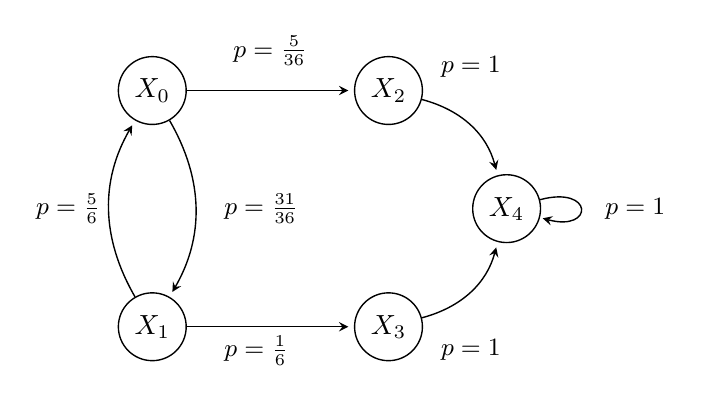
\begin{tikzpicture}[->, >= stealth, shorten >=2pt, line width=0.5pt, node distance=2cm]
  \node[circle, draw] (A) at (0, 3) {$X_0$};
  \node[circle, draw] (B) at (0, 0) {$X_1$};
  \node[circle, draw] (C) at (3, 3) {$X_2$};
  
  \node[circle, draw] (D) at (3, 0) {$X_3$};
  \node[circle, draw] (E) at (4.5, 1.5) {$X_4$};
  
  
  \begin{small}
    \path (A) edge [bend left]  node [left][right=0.25cm] {$p = \frac{31}{36}$} (B);
     \path (B) edge [bend left] node [left] {$p = \frac{5}{6}$} (A);
      \path (A) edge  node [left][above=0.2cm] {$p = \frac{5}{36}$} (C);
       \path (B) edge  node [left][below=0.3cm][right=-0.7cm] {$p = \frac{1}{6}$} (D);
        \path (C) edge [bend left] node [left][above=0.5cm] {$p = 1$} (E);
         \path (D) edge [bend right] node [left][below=0.5cm] {$p = 1$} (E);
         \path (E) edge [loop right] node [left] [right=0.2cm]{$p = 1$} (E);
   % \path (A) edge [bend left] node [below = 0.4cm] {$p = \frac{31}{36}\times\frac{5}{6}\times\frac{5}{36}$} (B);
    %\path (A) edge [bend right] node [below = 0.2cm] {$p = \frac{31}{36}\times\frac{5}{36}\times\frac{31}{36}$} (C);
    
    
  \end{small}
\end{tikzpicture}
}
    \caption{State diagram generated using LatexTikZ}
    \label{fig:Statediagramdiecoin}
\end{figure}
\\
Initial state vector\\
\begin{align}
\vec{S}_0 &= \myvec{ 1\\ 0\\0\\0\\0\\}
\end{align}
Transition matrix\\
\begin{align}
\vec{P} &= \myvec{
    0 & \frac{5}{6} & 0 & 0 & 0 \\
    \frac{31}{36} & 0 & 0 & 0 & 0 \\
    \frac{5}{36} & 0 & 0 & 0 & 0 \\
    0 & \frac{1}{6} & 0 & 0 & 0 \\
    0 & 0 & 1 & 1 & 1\\
}
\end{align}
Probablity of A winning in third throw given A starts first\\
\begin{align}
\vec{S}_1 &= \vec{P}\vec{S_0}\\
\vec{S_2} &= \vec{P}\vec{S_1}\\
\vec{S_3} &= \vec{P}\vec{S_2}\\
    &= \vec{P^3}\vec{S_0}\\
&= \myvec{
    \frac{775}{1296} & 0 & 0 & 0 & 0 \\
    \frac{4805}{7776} & 0 & 0 & 0 & 0 \\
    \frac{775}{7776} & 0 & 0 & 0 & 0 \\
    0 & \frac{155}{1296} & 0 & 0 & 0 \\
    \frac{61}{216} & \frac{61}{216} & 1 & 1 & 1
}
\myvec{ 1\\ 0\\0\\0\\0\\}\\
\vec{S_3} &= \myvec{0.597\\ 0.617\\0.099\\0\\0.282}\\
\vec{S_3}[2] &= 0.099
\end{align}



\end{enumerate}
